\section{Experiments}\label{chapter4}

\subsection{Noise}
Three kinds of noises, Gaussian noise, Poisson noise and Salt $&$ Pepper noise are implemented as follows.
\subsubsection{Gaussian Noise}
\begin{lstlisting}[caption= Gaussian Noise Design, label=matn1]
def normal(subVhat):
    """Design a Gaussian noise."""
    V_noise = np.random.normal(0, 80, subVhat.shape) #* np.sqrt(subVhat)
    V = subVhat + V_noise
    V[V < 0] = 0
    return V, V_noise
\end{lstlisting}

Random noises drawn from Gaussian distribution with 0 mean and 80 standard deviation are added to original images

\subsubsection{Poisson Noise}
\begin{lstlisting}[caption= Poisson Noise Design, label=matn1]
def possion(subVhat):
    """Design a Possion noise."""
    V = np.random.poisson(subVhat)
    V_noise = V-subVhat
    return V, V_noise
\end{lstlisting}

Random noises drawn from Poisson distribution with parameter to be 40.

\subsubsection{Salt and Pepper Noise}
\begin{lstlisting}[caption= Salt and Pepper Noise Design, label=matn1]
"""Design a salt and pepper noise where make some pixel value zeros."""
  # obtain one Image
  image = subVhat[:, 0]
  V_noise = np.random.randint(low=0, high=255, size=subVhat.shape, dtype=int)
  V = subVhat.copy()
  V[V_noise <= 20] = 0
  V[V_noise >= 230] = 255
  return V, V_noise
\end{lstlisting}

Salt and Pepper noises are added by drawing random integers from discrete uniform distribution of the interval $[$0, 255$)$

\subsubsection{Experiments Results}
The results of noise design are shown below:
\begin{figure}\label{noises}
	\centering
	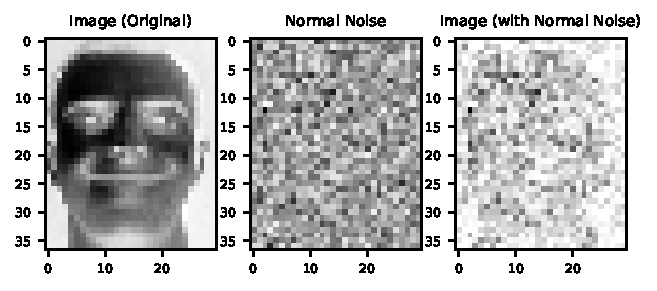
\includegraphics[scale=.8]{Noise_ORL_Normal_Comparison}\\ %replace these with jpg files with appropriate size
	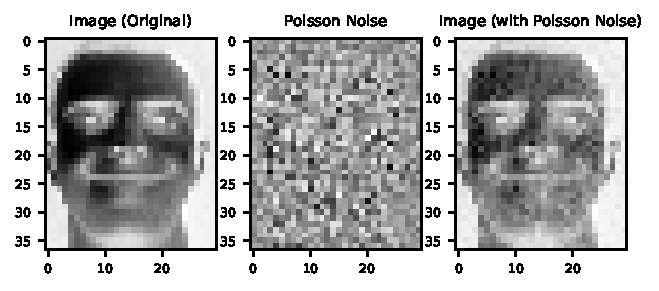
\includegraphics[scale=.8]{Noise_ORL_Poisson_Comparison}\\
	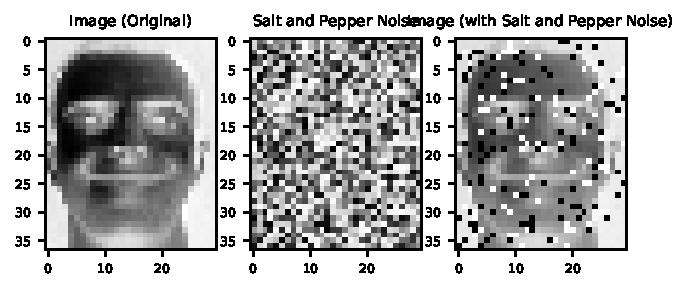
\includegraphics[scale=.8]{Noise_ORL_Salt_and_Pepper_Comparison}
	\caption{The original images (left) are corrupted by Gaussian Noise (top), Poisson Noise (middle), and Salt \& Pepper Noise (bottom). The corrupted images are shown on the right.}
	\label{fig:noise}
\end{figure}
